\section{\LARGE{Elettroforesi SDS-PAGE}}

\vspace{0.6cm}


\subsection{Sommario}

\subsubsection{Scopo}

Lo scopo di questa esperienza e' effettuare l'elettroforesi
delle proteine estratte nell'esperienza 10 tramite la
tecnica SDS-PAGE.

\subsubsection{Cenni teorici}

Solitamente l'elettroforesi ha la capacit\`a di separare le proteine secondo sia
la carica che la massa.
L'elettroforesi SDS-PAGE, che si effettua in gel di acrilammide, si differenzia
rispetto ad altre procedure in quanto la separazione delle proteine
avviene solo in base al solo peso molecolare, indipendentemente dalla carica.
Ci\`o \`e possibile grazie alla propriet\`a denaturante dell'SDS,
che permette di mantenere costante il rapporto massa-carica per ogni proteina denaturata.
L'SDS, acronimo di Laurilsolfato di sodio, e' un tensioattivo in grado di denaturare le proteine e
caricarle negativamente in modo proporzionale alla loro massa.

Il gel e' diviso in due parti, stacking gel e running gel. Lo stacking gel
ha lo scopo di allineare le proteine, portandole tutte allo stesso livello e per
questo contiene una percentuale minore di acrilammide.
Il running gel ha invece il compito di permettere alle proteine di separarsi a
seconda della carica.

\subsubsection{Strumenti e materiali utilizzati}

\begin{itemize}
\item Guanti in lattice
\item Provette Eppendorf (2ml)
\item Micropipette (100-1000 e 2-200 ml)
\item Falcon (50mL)
\item Carta bibula
\item Apparato per casting del gel elettroforetico
\end{itemize}

\subsubsection{Soluzioni e composti}

\begin{itemize}
\item Laemmli Sample Buffer 4X
\item Acrilammide/bis
\item 1,5M Tris-HCl, pH 8,8
\item Tris base
\item Glicina
\item 10\% soluzione SDS
\item 10\% ammonio persolfato
\item TEMED
\item isopropanolo
\item ddH20
\item Proteine da analizzare 20ug (estratte nell'esperienza 10)
\item Tris base
\item Glicina
\item 10\% soluzione SDS
\end{itemize}


\subsection{Procedimento}

\subsubsection{Caricamento delle proteine estratte}
\begin{itemize}
	\item Scongelare le proteine dell'esperienza precedente in ghiaccio.
	\item Calcolare, in base alla concentrazione, quanti $\mu$l di estratto
	utilizzare per caricare 15$\mu$g di proteine totali.
	\item Prima di caricare le proteine nei pozzetti, aggiungere il Laemmli Sample
	Buffer 4X, portandolo ad una concentrazione 1X.
	\item Bollire la miscela a 99°C per 10'.
	\item Caricare su un pozzetto.
\end{itemize}

\subsubsection{Corsa elettroforetica}
\begin{itemize}
	\item Connettere la camera di corsa con l'alimentatore.
	\item Impostare una ddp di 120V costanti.
	\item Verificare la corretta partenza della corsa.
	\item Attendere la fuoriuscita del fronte contrassegnato dal colorante utilizzato
	in fase di caricamento.
\end{itemize}

\begin{figure}[H]
	\centering
	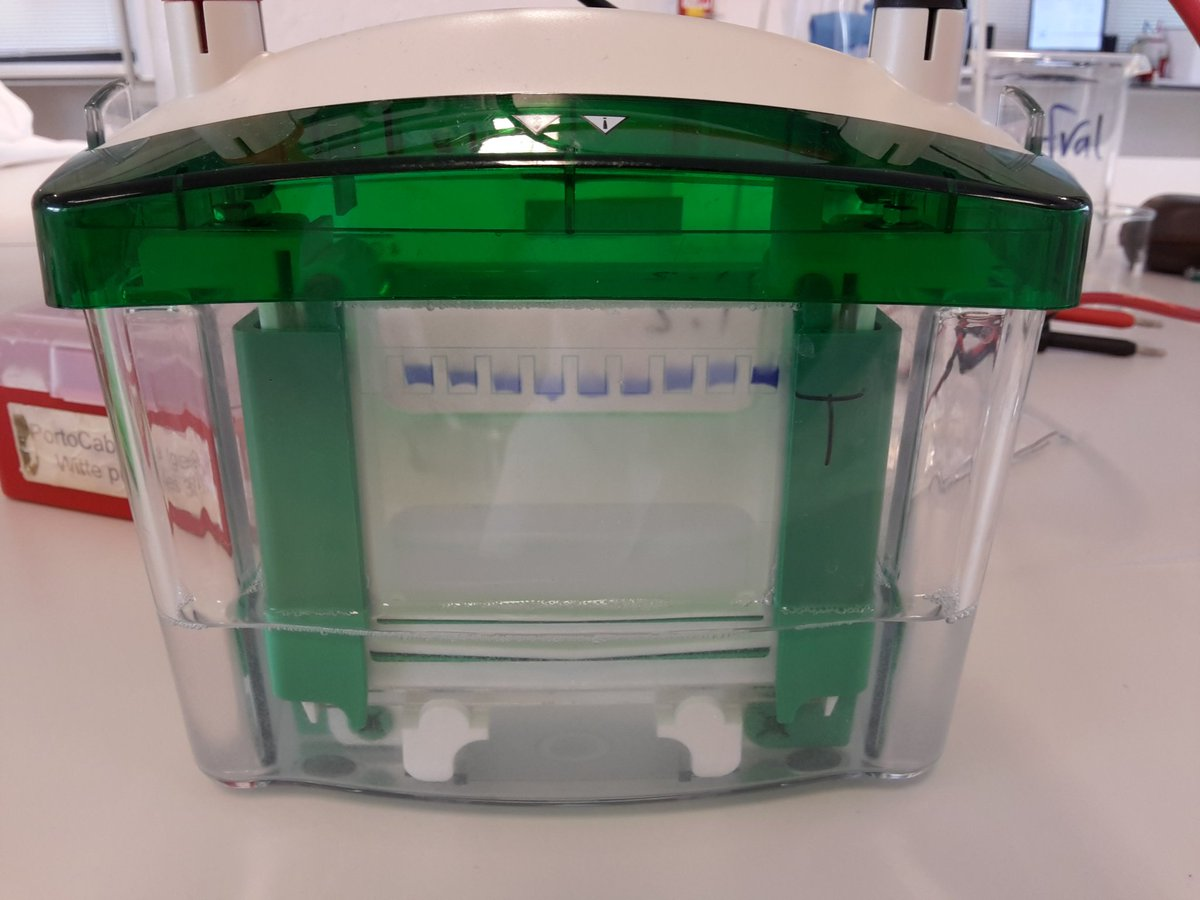
\includegraphics[width=0.3\textwidth]{./immagini/sds-page.jpg}
	\caption{Esempio di elettroforesi SDS-PAGE}
	\label{sds-page}
\end{figure}



\subsubsection{Preparazione del Running/Resolving gel}

\begin{tabular}{|l|l|l|} \hline
	& \textbf{Concentrazione} & \textbf{Quantit\'a} \\\hline
	Acrilammide/bis & 40\% & 3,2ml \\\hline
	1,5M Tris-HCl, pH 8,8 & 25\% & 2,0ml \\\hline
	SDS soluzione 10\% & 1\% & 0,8ml \\\hline
	Ammonio persolfato 10\% & 1\% & 0,8ml \\\hline
	TEMED & 0,1\% & 0,08ml \\\hline
	ddH$_2$O & \multicolumn{2}{c|}{a volume totale} \\\hline

	& \textbf{TOTALE} & 300ml \\\hline
\end{tabular}

\begin{enumerate}
	\item Predisporre l'apparato necessario al casting del gel elettroforetico.

	\item Miscelare tutti i componenti della tabella 1 in una Falcon da 50ml.

	\item Distribuire velocemente la miscela tra i vetri dell'apparato, \`e importante
	tenere l'eccesso del gel all'interno della Falcon, per stabilire quando il gel
	si sar\`a solidificato.

	\item Stratificare sino a riempimento con alcol isopropilico.
	Questa fase \`e necessaria per limitare il contatto con l'aria
	del gel che si sta solidificando e contemporaneamente	permettere
	un livellamento del gel grazie al peso dell'alcol.
	\`E importante notare che in questa fase l'alcol e
	il gel non si mescolano.

	\item Attendere la polimerizzazione (confermata dalla quantit\`a di
	gel lasciata nella Falcon)
\end{enumerate}

\subsubsection{Preparazione dell'Electrode Running Buffer 10X}
\begin{itemize}
	\item Preparare l'Electrode Running Buffer utilizzando
	le seguenti soluzioni:\\
	\begin{tabular}{|l|l|l|} \hline
		& \textbf{Concentrazione} & \textbf{Quantit\'a} \\\hline
		Tris base & 3\% & 9ml \\\hline
		Glicina & 14,4\% & 43,2ml \\\hline
		SDS soluzione 10\% & 1\% & 3ml \\\hline
		& \textbf{TOTALE} & 300ml \\\hline
	\end{tabular}
\end{itemize}

\subsubsection{Preparazione dello stacking gel}

\begin{tabular}{|l|l|l|} \hline
	& \textbf{Concentrazione} & \textbf{Quantit\'a} \\\hline
	Acrilammide/bis & 61\% & 3,05ml \\\hline
	1,5M Tris-HCl, pH 8,8 & 25\% & 1,25ml \\\hline
	10\% soluzione SDS & 1\% & 0,05ml \\\hline
	10\% ammonio persolfato & 1\% & 0,05ml \\\hline
	TEMED & 0,2\% & 0,01ml \\\hline
	ddH20 & \multicolumn{2}{c|}{a volume totale} \\\hline
	& \textbf{TOTALE} & 5ml \\\hline
\end{tabular}

\begin{itemize}
	\item Miscelare tutti i componenti della tabella in una Falcon
	da 50ml.
	\item Aliquotare rapidamente la miscela tra i vetri del gel, tenendo
	l'eccesso nella Falcon per confronto.
	\item Inserire il pettine per permettere la formazione dei pozzetti
	di caricamento.
	\item Attendere la polimerizzazione del gel.
\end{itemize}

% \begin{enumerate}


	% \begin{figure}[H]
	% 	\centering
	% 	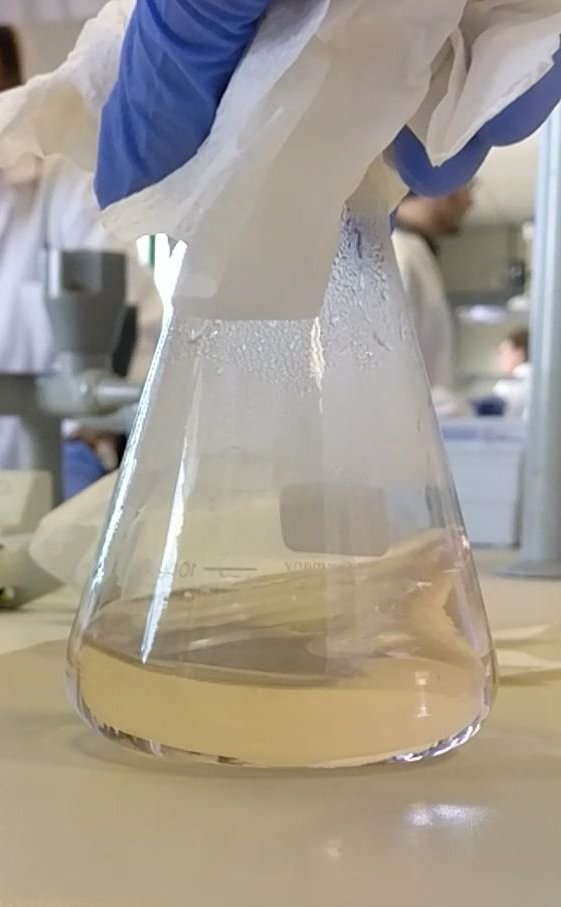
\includegraphics[width=0.3\textwidth]{./immagini/agarosio.jpg}
	% 	\caption{Mescolamento della soluzione con agarosio}
	% 	\label{agarosio}
	%
	% \end{figure}


% \end{enumerate}
\subsubsection{Colorazione del gel}
\begin{itemize}
\item Smontare i vetri che racchiudono il gel di corsa.
\item Lavara i gel per 3 volte da 5' ciascuna in ddH$_2$O.
\item Porre i gel in 10ml di Comassie Blue Staining.
\item Lasciar colorare per circa 1h.
\item Lavare i gel 5 volte in ddH$_2$O.
\end{itemize}


\subsection{Risultati e Conclusioni}

In questa esperienza abbiamo imparato come svolgere una tecnica
molto utilizzata in biologia molecolare, che permette la separazione
delle proteine in base alla loro massa.
Purtroppo nel nostro caso, a causa di un errore di concentrazione
dell'Electrode Running Buffer, non \`e stato possibile ottenere
risultati soddisfacenti.
